
\section{Introduction}

\subsection{License and Copyright}

InsightCAE is free software; you can redistribute it and/or modify it under the terms of version 2 of the GNU General Public License\footnote{\url{http://www.gnu.org/licenses/old-licenses/gpl-2.0.html}} as published by the Free Software Foundation. You accept the terms of this license by distributing or using this software.

This manual is Copyright (c) 2017 silentdynamics GmbH.

Permission is granted to copy, distribute and/or modify this document under the terms of the GNU Free Documentation License, Version 1.3 or any later version published by the Free Software Foundation; with no Invariant Sections, no Front-Cover Texts, and no Back-Cover Texts. A copy of the license is included in the section entitled "GNU Free Documentation License".

\subsection{Contributors}

The following people have so far contributed to InsightCAE:
\begin{itemize}
\item Hannes Kröger (silentdynamics GmbH)
\item Johann Turnow (silentdynamics GmbH)
%%
%% Please add yourself here, if you made any contribution
%%
\end{itemize}

Is you want to get involved in the development, please feel invited to do so!
We greatly appreciate any contribution and we would very much like to add you to the above list.

If you made some modification or addition to the code, which you would like to be merged into the main development line, please consider to send us a pull request\footnote{\url{https://help.github.com/en/github/collaborating-with-issues-and-pull-requests/about-pull-requests}}.

\subsection{About InsightCAE}

InsightCAE is a workbench for Computer-Aided Engineering. Individual open source projects often meet only subtasks in analysis process. To automate repetitive computational tasks, a combination of several open source engineering software tools is often required. In order to use open source software productive and efficient for everyday tasks, the analysis automation framework InsightCAE was created.

InsightCAE serves as a framework for the implementation of analysis procedures. The objective is to provide interfaces to the tools and simulation programs that are needed for a specific computing task.

\subsection{Features and Highlights}

InsightCAE's objective is to create automated analysis workflows.
The high level API resides in the core "toolkit" library.
Automated workflows usually involve different external programs and utilities.
For the realization of automated workflows, it is sometimes required, to create add-ons to these external programs.
Thus InsightCAE is also a container for add-ons to other programs.

\begin{itemize}
\item InsightCAD script-based, fully parametric CAD

\begin{itemize}
    \item OpenCASCADE geometry kernel
    \item assemblies, constraint-based sketches, part library, drawing export
\end{itemize}

\item OpenFOAM add-ons (schemes, boundary conditions, models, ...)
\item Pre- \& Postprocessing tool (OpenFOAM Case Builder)
\item analysis workflow automation tools (GUI)
\end{itemize}

\subsection{Reading this Manual}


\subsection{Recommendations for Working with Shell-based Tools in Linux}

Sometimes it is necessary to execute tools in a bash shell, e.g. because no GUI for it is available. And often it is easier to keep an overview in graphical file manager.
Having a console window open together with a file manager window at the same time is an obvious solution but to do so for many cases at a time may easily confuse the desktop. 

Here are two useful hints to solve this issue:
 
\begin{enumerate}

 \item The KDE file manager \textbf{dolphin} offers the possibility to display a console in the lower half of the window (figure \ref{fig:dolphin}). The working directory is synchronized with the directory shown in the graphical window by injection of \textbf{cd} commands. Vice versa, when the working directory is changed in the shell, the graphical display is updated as well.
 
 \begin{figure}[h!]
 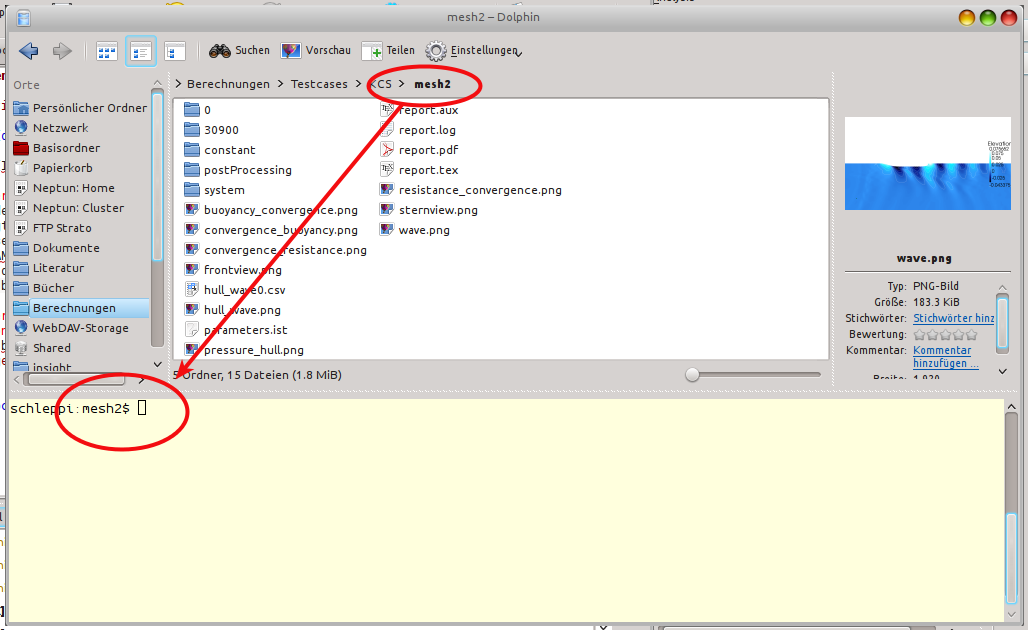
\includegraphics[width=\linewidth]{figs/intro/dolphin_with_terminal} 
 \caption{Dolphin file manager with embedded terminal}
 \label{fig:dolphin}
 \end{figure}

 \item There is a Norton-Commander-like file manager named \textbf{krusader} (figure \ref{fig:krusader}). It offers the same functionality regarding the embedded terminal but a more flexible way of displaying multiple folders. In addition to the two list view on the left and right, multiple tabs for folders can be added in each list view. And there is also a rich interface to define custom commands and file associations.
 
 \begin{figure}[h!]
 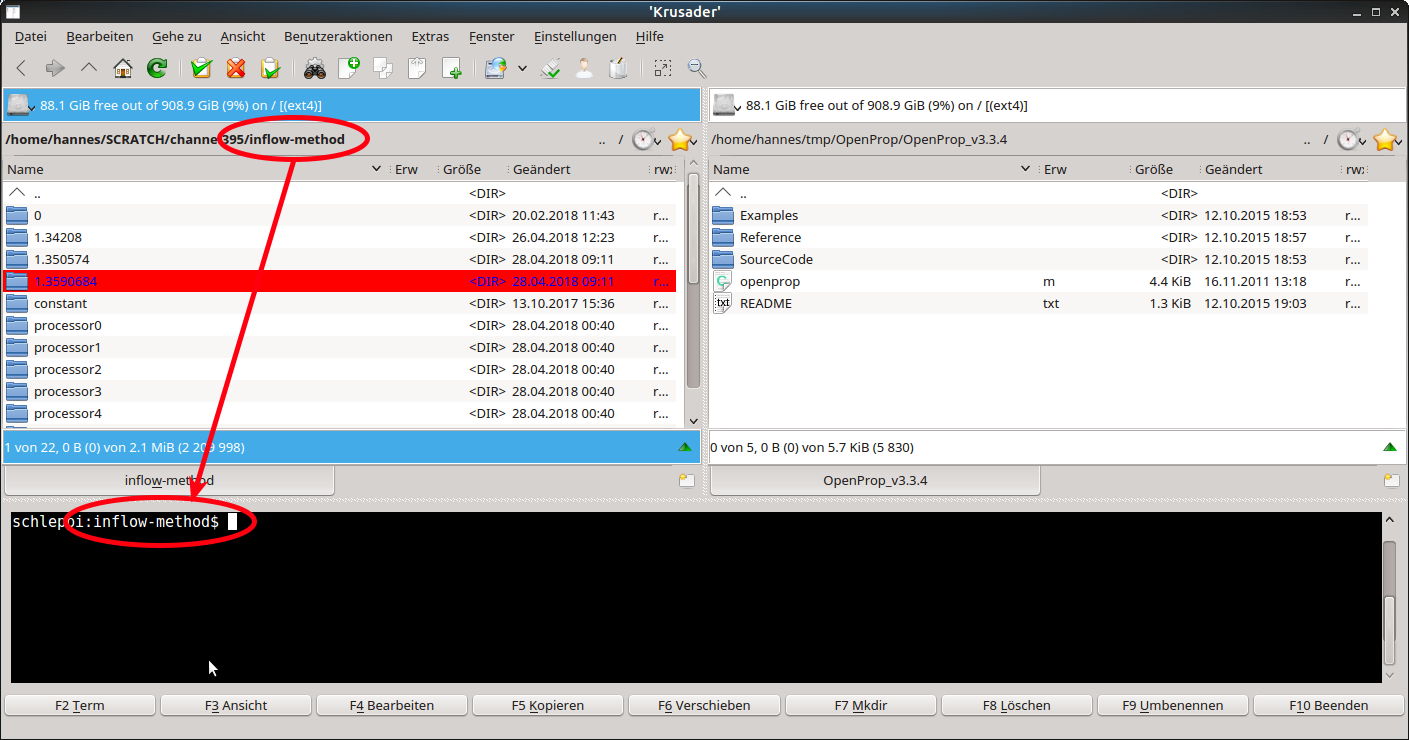
\includegraphics[width=\linewidth]{figs/intro/krusader_with_terminal}
 \caption{Krusader file manager with embedded terminal}
 \label{fig:krusader}
 \end{figure}
 
\end{enumerate}


\subsection{Resources}

\subsubsection{In the Web}

\begin{itemize}
\item Source Code Repository \url{https://github.com/hkroeger/insightcae}
\item Issue Tracker \url{https://github.com/hkroeger/insightcae/issues}
\item Web Forum \url{https://groups.google.com/forum/#!forum/insightcae}
\end{itemize}

\subsubsection{Reporting Bugs and Feature Requests}

Please use the issue tracker \url{https://github.com/hkroeger/insightcae/issues} to report any bugs.

We also monitor the web forum \url{https://groups.google.com/forum/#!forum/insightcae} for questions or feature requests.

\subsubsection{Getting Professional Help and Support}

Beyond the web resources above, silentdynamics GmbH offers commercial support\footnote{\url{http://silentdynamics.de/en/oss-cae/}} for professional users of InsightCAE. Automated analyses according to customer needs and specifications are implemented  by creating new specialized modules for Insight CAE.
Typical support contracts include also user training and continuous customization and updating of InsightCAE and its add-ons.


\section{Obtaining InsightCAE}

\subsection{Installation using Linux Package Manager}

We provide installation packages for Ubuntu-based Linux distributions. We specifically support the latest Ubuntu LTS distibution.

The packages are held in our repository. To install them, first add the silentdynamics apt repository and the associated key by executing:

\begin{lstlisting}[language=bash]
$ sudo apt-key adv --fetch-keys http://downloads.silentdynamics.de/SD_REPOSITORIES_PUBLIC_KEY.gpg
$ sudo add-apt-repository http://downloads.silentdynamics.de/ubuntu
$ sudo apt-get update
\end{lstlisting}

Then, install the software by executing

\begin{lstlisting}[language=bash]
$ sudo apt-get install insightcae-base
\end{lstlisting}


Note:
in Ubuntu 18.04 LTS, the file \file{/etc/ImageMagick-6/policy.xml} needs to be modified. Otherwise the charts in the reports will not be created properly.
Find the line
\begin{lstlisting}[language=xml]
<policy domain="coder" rights="none" pattern="PDF" />
\end{lstlisting}

and change it to
\begin{lstlisting}[language=xml]
<policy domain="coder" rights="read|write" pattern="PDF" />
\end{lstlisting}

\subsection{Installation on Windows}
Currently, there is no native Windows version of InsightCAE available.
However, it can be run in Windows 10 Enterprise (64 bit only) or Windows Server using the "Linux Subsystem for Windows" (WSL). This should be preferred over virtualization solutions like VirtualBox, because it offers the best parallel performance. The processes share the memory with the Windows processes and the files are stored in the Windows file system. Various X servers are available for graphical output under Windows; Xming is used below.

To use this solution, the Linux subsystem must first be activated. Adminstration privileges are required. It is done by the following steps:

Start Windows PowerShell as an administrator (right-click on Start menu \textgreater "PowerShell (Admin)") and execute:
\begin{lstlisting}[language=bash]
> Enable-WindowsOptionalFeature -Online -FeatureName Microsoft-Windows-Subsystem-Linux
\end{lstlisting}
Restart the computer when prompted.

Download the Linux image:
\begin{lstlisting}[language=bash]
> Invoke-WebRequest -Uri https://aka.ms/wsl-ubuntu-1804 -OutFile ~/Ubuntu.zip -UseBasicParsing
\end{lstlisting}

Unpack:
\begin{lstlisting}[language=bash]
> Expand-Archive ~/Ubuntu.zip c:\Distros\Ubuntu
\end{lstlisting}

Configuring the Linux System:
Switch to user "root":
\begin{lstlisting}[language=bash]
> c:\Distros\Ubuntu\ubuntu.exe config --default-user root
\end{lstlisting}

Set the password of the user "user":
\begin{lstlisting}[language=bash]
> c:\Distros\Ubuntu\ubuntu.exe
# passwd user
\end{lstlisting}

Install InsightCAE with OpenFOAM:

\begin{lstlisting}[language=bash]
# echo deb http://downloads.silentdynamics.de/ubuntu bionic main > /etc/apt/sources.list.d/sd.list
# apt-key adv --fetch-keys http://downloads.silentdynamics.de/SD_REPOSITORIES_PUBLIC_KEY.gpg
# apt-get update
# apt-get install insightcae-base
\end{lstlisting}

Switch back to standard user ("user"):

\begin{lstlisting}[language=bash]
> c:\Distros\Ubuntu\ubuntu.exe config --default-user user
\end{lstlisting}

Add the file \file{c:{\textbackslash}Distros{\textbackslash}Ubuntu{\textbackslash}ubuntu.exe} to the start bar

Then install the Xming server for graphical output:

Download Xming-Installer\footnote{e.g. \url{https://sourceforge.net/projects/xming/files/Xming/6.9.0.31/Xming-6-9-0-31-setup.exe}}, then execute the installer:
\begin{itemize}
\item Check: "Install quick launch icon"
\item Allow network access after installation
\end{itemize}

Set the DISPLAY variable in the Bash environment
\begin{lstlisting}[language=bash]
$ sudo -i
# echo "export DISPLAY=:0" >> /etc/profile.d/xming.sh
# exit
\end{lstlisting}

\paragraph{Usage}
First start "Xming" X-Server,
then start Ubuntu Bash command line.
Execute the application in the shell, e.g. the InsightCAE Workbench:
\begin{lstlisting}[language=bash]
$ workbench
\end{lstlisting}

\subsection{Building from Sources}

The source code of InsightCAE is hosted at Github. 
Cloning a working copy constitutes the best way to get updates and the latest bug fixes.

Alternatively, you can download snapshot archives from github, if you don't want to bother with a git client.
In this case, just replace the cloning step below with unpacking the archive.

First, get the the sources by cloning the git repository:
\begin{lstlisting}[language=bash]
$ git clone https://github.com/hkroeger/insightcae.git insight-src
\end{lstlisting}

CMake is utilized for managing the build. 
The preferred way is to build the software out of source in a separate build directory. Create a build directory, then configure the build using e.g. ccmake and finally build using make:

\begin{lstlisting}[language=bash]
$ mkdir insight && cd insight
$ ccmake ../insight-src
\end{lstlisting}
In the CMake GUI, you may need to change paths or adapt settings. Please refer to the CMake documentation\footnote{\url{https://cmake.org/cmake/help/latest/guide/tutorial/index.html}} on how to use CMake.
The biggest difficulty will probably be, to provide all the software packages, on which InsightCAE depends.

The final step in CMake is, to generate the Makefiles. Once this is done without errors, start the compilation of the project by executing:

\begin{lstlisting}[language=bash]
$ make
\end{lstlisting}

To work with InsightCAE, some environment variables are needed to be set up. A script is provided therefore. It can be parsed e.g. in your \file{\textasciitilde/.bashrc} script by adding to the end:

\begin{lstlisting}[language=bash]
source /path/to/insight/bin/insight_setenv.sh
\end{lstlisting}
